% Sec. Testbed Design
\section{Testbed Design}
\label{sec:design}
SCooP-iT consists of two mobile agents and three infrastructure
agents connected to a single access point, with an additional host
that extracts channel state. In IoT terms each agent is a node that
senses, computes, and communicates: the mobile agents are mobile IoT
nodes, the masts fixed ones, and the access point the shared network
whose behavior the testbed measures. Fig.~\ref{fig:overview} shows a recording
scenario with the agents placed in the map frame and the measured
links between them. \todo{Redraw Fig.~\ref{fig:overview} per the plan:
floor plan with agents in the map frame, links colored by measured RTT
or RSSI, and a strip below with one shared timeline of sensor frames,
link samples, and CSI. It should say ``one clock, one frame, every
link'' without text.}

\begin{figure}[t]
\centering
\fbox{\parbox[c][5cm][c]{0.95\columnwidth}{\centering
\todo{Fig.~1: one window of \texttt{coop\_2} on one timeline. Top: floor
plan with both robots' paths and the masts in the map frame, the
robot-to-AP paths coloured by Fresnel clearance. Below, stacked on a
shared time axis: clearance, RSSI, RTT, goodput, and each
\SI{1.5}{\mega\byte} message's predicted arrival against the
\SI{100}{\milli\second} frame boundary.}}}
\caption{SCooP-iT in one window: agents in one map frame, every link
measured, one clock. Where the map shows the path obstructed, the
signal drops, goodput falls, and large messages miss their frame.}
\label{fig:overview}
\end{figure}


\subsection{Agents}
\texttt{mobile\_1}, the LiDAR robot, is an AgileX Scout Mini equipped
with an Ouster OS1-64 LiDAR, a ZED~2i stereo camera with an integrated IMU,
two IWR6843 mmWave radars, and an RTL8852BU Wi-Fi interface. It also
carries \texttt{sniffer}, a Raspberry Pi~4 whose BCM43455c0 chipset is
used for CSI extraction. \texttt{mobile\_2}, the RGB-D cart, is a
pushcart equipped with an Ouster OS1-128 LiDAR, a RealSense D455 RGB-D
camera with IMU, an on-board visual SLAM pipeline, and a Wi-Fi interface \todo{Add Radar
(?)}. Each infrastructure mast, \texttt{infra\_N}, carries an Arducam
RGB camera, an IWR6843 radar, and a Raspberry Pi whose on-board
BCM43455 serves as the wireless interface. The sensor models, rates,
and resolutions are listed in Table~\ref{tab:sensors}; compute,
storage, and cost per agent class are given in Table~\ref{tab:bom}.
The three classes are deliberate: the LiDAR robot builds the reference
map, the cart represents the low-cost agents a deployed team contains
and that a reference must localize without a LiDAR, and the masts
provide the elevated, persistent vantage no mobile node can sustain.

\begin{figure*}[t]
\centering
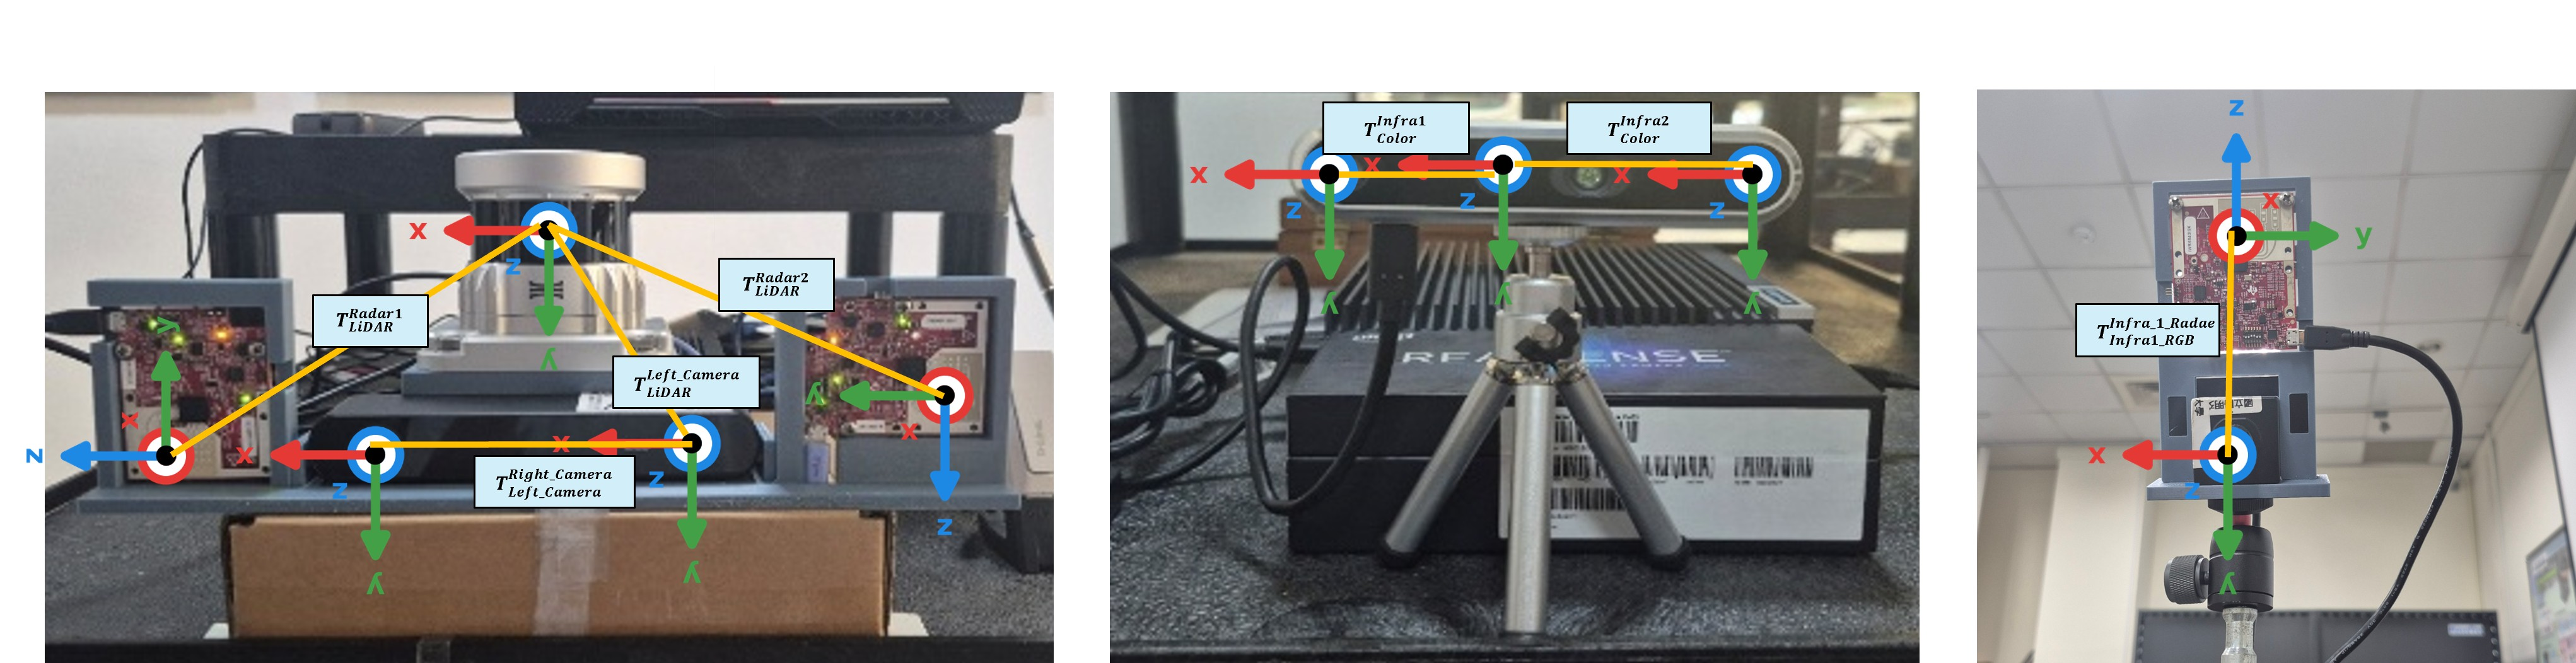
\includegraphics[width=\textwidth]{figs/fig02_platforms.jpg}
\caption{Platforms and frames. Axes mark each sensor frame (x red,
y green, z blue); yellow arrows are the extrinsic transforms
estimated in Sec.~\ref{sec:alignment}. \texttt{mobile\_1} uses
\texttt{base\_link} as origin (not shown here), \texttt{mobile\_2} its LiDAR, and the
infrastructure rig its camera.}
\label{fig:platforms}
\end{figure*}

\begin{table}[t]
\centering
\caption{Sensing per agent class (full specification in the
supplementary material).}
\label{tab:sensors}
\footnotesize
\setlength{\tabcolsep}{3pt}
\begin{tabularx}{\columnwidth}{@{}l>{\raggedright\arraybackslash}Xl@{}}
\toprule
Agent & Sensor & Rate \\
\midrule
\multirow{5}{*}{\texttt{mobile\_1}} & Ouster OS1-128 / OS0-64 LiDAR & \SI{10}{\hertz} \\
 & ZED 2i stereo (1920$\times$1080) + IMU & 30 / \SI{400}{\hertz} \\
 & 2$\times$ TI IWR6843ISK \SI{60}{\giga\hertz} radar & \SI{10}{\hertz} \\
 & RTL8852BU 802.11ac Wi-Fi & 5 / \SI{100}{\hertz} \\
 & \texttt{sniffer}: RPi 4B BCM43455c0 CSI (242 sc.) & $\sim$\SIrange{100}{140}{\hertz} \\
\midrule
\multirow{3}{*}{\texttt{mobile\_2}} & RealSense D455 RGB-D (1280$\times$800) & \SI{30}{\hertz} \\
 & IMU BMI055; on-board visual SLAM & 200 / \SI{30}{\hertz} \\
 & 802.11ac Wi-Fi & 5 / \SI{100}{\hertz} \\
\midrule
\multirow{3}{*}{\texttt{infra\_N}} & Arducam B0495 RGB (1920$\times$1200) & \SI{30}{\hertz} \\
 & TI IWR6843ISK radar & \SI{10}{\hertz} \\
 & RPi 4B BCM43455 Wi-Fi & 5 / \SI{100}{\hertz} \\
\bottomrule
\end{tabularx}
\end{table}


\begin{table}[t]
\centering
\caption{Bill of materials and per-site setup effort. \todo{Fill costs and effort.}}
\label{tab:bom}
\footnotesize
\setlength{\tabcolsep}{4pt}
\begin{tabularx}{\columnwidth}{@{}l>{\raggedright\arraybackslash}Xr@{}}
\toprule
Agent class & Main components & Cost \\
\midrule
LiDAR robot (\texttt{mobile\_1}) & Scout Mini, Ouster OS1-64, ZED 2i, 2$\times$ IWR6843ISK, Jetson AGX Orin, RTL8852BU, RPi 4B sniffer & \todo{} \\
RGB-D cart (\texttt{mobile\_2}) & Pushcart, Ouster OS1-128, RealSense D455, compute \todo{}, Wi-Fi & \todo{} \\
Infrastructure mast (\texttt{infra\_N}) & Mast, Arducam B0495, IWR6843ISK, RPi 4B & \todo{} \\
Network & 1 access point (802.11ac, VHT-80), rangefinder, printed ChArUco boards & \todo{} \\
\midrule
\multicolumn{3}{@{}l}{\emph{Per new site:} mapping session \todo{min}; \todo{N} boards; \todo{N} rangefinder distances; second pass optional} \\
\bottomrule
\end{tabularx}
\end{table}


\subsection{Network}
All agents associate to a single access point on channel 149 (VHT-80,
\SI{5745}{\mega\hertz}); no ad hoc or mesh mode is used, and power
save is disabled on all transmitters. The transmitter settings are
imposed by the CSI receiver: a 1$\times$1 802.11ac configuration.
802.11ax is disabled, since the receiver cannot demodulate HE frames
and would capture only control frames, and the number of spatial
streams is fixed to one, since a single-antenna receiver cannot
separate a two-stream transmission. The measured single-stream
capacity is \numrange{275}{282}\,Mbit/s uplink and
\numrange{598}{676}\,Mbit/s downlink per mobile agent.

\subsection{Design Decisions}
\label{sec:decisions}
Four decisions make SCooP-iT a testbed rather than a hardware list.

\emph{The link is measured, not used to carry sensor data.} Each unit
records locally; no sensor stream traverses the wireless network
before reaching disk. Measurement and transport stay separate, so any
method's traffic can be replayed afterwards (Sec.~\ref{sec:replay})
without the recording having been shaped by one method. The only
traffic the testbed itself places on the link is clock synchronization
and the active probes of Sec.~\ref{sec:link}, present in every run and
therefore part of the channel that is measured.

\emph{Single stream, 802.11ax off.} The 1$\times$1 CSI receiver
requires it. It also keeps capacity governed by geometry rather than
by scattering richness, which two-stream capacity depends on and which
a map does not capture.

\emph{Survey and cooperation modes.} In survey mode each agent owns
the whole channel; in cooperation mode several agents run their active
tests at the same time by design. Contention becomes a controlled knob
instead of an accident, and its effect is measurable: RTT moves from
\SI{3.3}{\milli\second} idle to \SIrange{60}{109}{\milli\second} under
load (Sec.~\ref{sec:link}).

\emph{Fixed sensor rigs.} In each agent a fixed rig compounds the
sensors (Fig.~\ref{fig:platforms}), so calibration is done once and
each extrinsic can be validated on observations that did not enter it
(Sec.~\ref{sec:alignment}). The sensors of each platform are expressed
in that platform's origin frame: \texttt{base\_link} for
\texttt{mobile\_1}, so that poses relate to wheel odometry and control;
the LiDAR for \texttt{mobile\_2}, which has no robot body; and the
camera for the masts, which carry no LiDAR.

The remaining knobs a user controls are the number and class of
agents, the infrastructure placement, the trajectory paradigm
(concurrent, intersecting, or rendezvous), and agent speed.

\subsection{Recording}
\label{sec:recording}
Each unit records one bag containing what its sensors and interfaces
produce, and nothing else (topic list in the supplementary material): Ouster packets
with the sensor's metadata message, which allows lossless re-decoding
through the vendor driver at any later time; images and IMU samples;
radar detections; the full on-board visual SLAM output of
\texttt{mobile\_2}, including the drifting visual-odometry path, the
loop-closed path, and the tracker status; the wireless and clock topics
of Sec.~\ref{sec:link} on the same timeline as the sensor topics; and
the raw Nexmon CSI frames on \texttt{sniffer}. Decoded clouds,
reference poses, and parsed CSI do not exist at recording time; they
are produced by the post-processing pipeline (data-flow diagram in the
supplementary material), which decodes the streams, computes the reference poses
(Sec.~\ref{sec:gt}), parses the link and CSI logs, and merges all units
into one MCAP per run on the common timebase, with each unit's original
stamp preserved in the MCAP publish time. Every stage is scripted and
released so that the products can be regenerated.

% Topics table and data-flow figure live in supplementary.tex
